%=========================================================================
% Appendix Section: Mathematical Foundations
% =========================================================================
\begin{appendices}
  \section{Mathematical Notation}
  \label{app:math_notation}

  This section provides a reference for the mathematical notation used throughout this thesis.

  \begin{table}[htbp]
    \centering
    \caption{Mathematical Notation Used in This Thesis}
    \label{tab:math_notation}
    \resizebox{width=0.8\textwidth}{!}{%
      \begin{tabular}{p{0.28\textwidth}p{0.68\textwidth}}
        \toprule
        \textbf{Notation}                           & \textbf{Description}                                                                 \\
        \midrule
        \multicolumn{2}{l}{\textbf{Basic Notation}}                                                                                        \\
        \midrule
        $\bm{x}$, $\bm{y}$, $\bm{z}$                & Bold lowercase letters denote vectors                                                \\
        $W$, $A$, $Q$                               & Uppercase letters denote matrices                                                    \\
        $x_i$ or $(\bm{x})_i$                       & Subscript $i$ denotes the $i$-th element of vector $\bm{x}$                          \\
        $W_{ij}$                                    & Subscripts $i,j$ denote the element at row $i$, column $j$ of matrix $W$             \\
        $\bm{h}_t$                                  & Subscript $t$ typically denotes time step or sequence position                       \\
        $\mathbb{R}^n$                              & $n$-dimensional Euclidean space                                                      \\
        $\hat{y}$                                   & Predicted value (in contrast to true value $y$)                                      \\
        \midrule
        \multicolumn{2}{l}{\textbf{Mathematical Operations}}                                                                               \\
        \midrule
        $\odot$                                     & Hadamard (element-wise) product                                                      \\
        $[\bm{a};\bm{b}]$                           & Vertical concatenation of vectors $\bm{a}$ and $\bm{b}$                              \\
        $||\bm{x}||_p$                              & $L_p$ norm of vector $\bm{x}$                                                        \\
        $\nabla J(\theta)$                          & Gradient of function $J$ with respect to parameters $\theta$                         \\
        $d_{\text{Euclidean}}(\bm{a},\bm{b})$       & Euclidean distance between vectors $\bm{a}$ and $\bm{b}$                             \\
        $\text{CosineSimilarity}(\bm{a},\bm{b})$    & Cosine similarity between vectors $\bm{a}$ and $\bm{b}$                              \\
        \midrule
        \multicolumn{2}{l}{\textbf{Neural Network Components}}                                                                             \\
        \midrule
        $\sigma(\cdot)$                             & Sigmoid activation function                                                          \\
        $\tanh(\cdot)$                              & Hyperbolic tangent activation function                                               \\
        $\text{ReLU}(\cdot)$                        & Rectified Linear Unit activation function                                            \\
        $\text{softmax}(\bm{z})$                    & Softmax function applied to vector $\bm{z}$                                          \\
        $\vec{\bm{h}}_t$, $\cev{\bm{h}}_t$          & Forward and backward hidden states in Bi-LSTM                                        \\
        $\bm{h}_{\text{mean\_pool}}$                & Result of mean pooling operation on sequence                                         \\
        $\bm{h}_{\text{max\_pool}}$                 & Result of max pooling operation on sequence                                          \\
        $\bm{\gamma}$, $\bm{\beta}$                 & Scale and shift parameters in normalization layers                                   \\
        \midrule
        \multicolumn{2}{l}{\textbf{Optimization}}                                                                                          \\
        \midrule
        $\eta$                                      & Learning rate in optimization algorithms                                             \\
        $\lambda$                                   & Regularization strength parameter                                                    \\
        $\epsilon$                                  & Small constant added for numerical stability                                         \\
        $\bm{m}_t$, $\bm{v}_t$                      & First and second moment estimates in Adam optimizer                                  \\
        $\hat{\bm{m}}_t$, $\hat{\bm{v}}_t$          & Bias-corrected moment estimates in Adam optimizer                                    \\
        \midrule
        \multicolumn{2}{l}{\textbf{Loss Functions and Performance Metrics}}                                                                \\
        \midrule
        $\text{BCE}$                                & Binary Cross-Entropy loss function                                                   \\
        $\text{MSE}$                                & Mean Squared Error metric                                                            \\
        $\text{MAE}$                                & Mean Absolute Error metric                                                           \\
        $\text{MAPE}$                               & Mean Absolute Percentage Error metric                                                \\
        $\text{Precision}$                          & Precision metric in binary classification                                            \\
        $\text{Recall}$                             & Recall (sensitivity) metric in binary classification                                 \\
        $\text{F1}$                                 & F1-score, harmonic mean of precision and recall                                      \\
        $AUC$                                       & Area Under the Curve metric for binary classification                                \\
        $ROC$                                       & Receiver Operating Characteristic curve                                              \\
        $TPR$, $FPR$                                & True Positive Rate and False Positive Rate                                           \\
        $TP$, $TN$, $FP$, $FN$                      & True Positive, True Negative, False Positive, False Negative counts                  \\
        \midrule
        \multicolumn{2}{l}{\textbf{Statistical Concepts}}                                                                                  \\
        \midrule
        $\mu$, $\sigma^2$                           & Mean and variance of a distribution                                                  \\
        $\mathcal{N}(\mu,\sigma^2)$                 & Normal (Gaussian) distribution with mean $\mu$ and variance $\sigma^2$               \\
        $\text{UCL}$, $\text{LCL}$                  & Upper and Lower Control Limits in statistical process control                        \\
        $p$                                         & Proportion (typically of anomalies) in statistical process control                   \\
        $H_0$                                       & Null hypothesis in statistical testing                                               \\
        $\alpha$                                    & Significance level in statistical testing                                            \\
        $S_{obs}$                                   & Observed test statistic in permutation testing                                       \\
        $N$                                         & Number of permutations in permutation testing                                        \\
        $p$-value                                   & Probability of observing test statistic at least as extreme as $S_{obs}$ under $H_0$ \\
        $RR$                                        & Rejection rate of null hypothesis                                                    \\
        \midrule
        \multicolumn{2}{l}{\textbf{Feature Engineering}}                                                                                   \\
        \midrule
        $x_{\sin}$, $x_{\cos}$                      & Sine and cosine transformations of cyclical feature $x$                              \\
        $P$                                         & Period of cyclical feature in time encoding                                          \\
        $\mathcal{F}_c$                             & Feature subset in feature selection methods                                          \\
        \midrule
        \multicolumn{2}{l}{\textbf{Attention Mechanism}}                                                                                   \\
        \midrule
        $Q$, $K$, $V$                               & Query, Key, and Value matrices in attention mechanism                                \\
        $d_k$                                       & Dimension of key vectors in attention mechanism                                      \\
        \midrule
        \multicolumn{2}{l}{\textbf{Dataset Notation}}                                                                                      \\
        \midrule
        $\mathcal{D}$                               & Dataset or distribution                                                              \\
        $\mathcal{D}_{train}$, $\mathcal{D}_{test}$ & Training and testing datasets                                                        \\
        $\mathcal{D}_{real}$, $\mathcal{D}_{sim}$   & Real-world and simulation datasets                                                   \\
        \bottomrule
      \end{tabular}%
    }
  \end{table}

  \section{Mathematical Foundations}
  \label{app:math_foundations}

  This appendix provides formal definitions and illustrations for the core mathematical functions and operations referenced in the theoretical foundations chapter (Section~\ref{sec:rnn} onwards), as well as other relevant mathematical concepts and techniques commonly encountered in machine learning, deep learning, optimization, and data handling that are pertinent to the methods employed in this thesis. % Adjust Section ref if needed


  % -------------------------------------------------------------------------
  \subsection{Basic Notation and Operations}
  % -------------------------------------------------------------------------
  % (Content from previous version - vectors, matrices, basic ops...)
  As established at the beginning of the chapter, vectors are denoted by bold lowercase letters (e.g., \( \bm{z} \)) and matrices by uppercase letters (e.g., \( W \)). Vectors are assumed to be column vectors unless otherwise specified.

  \paragraph{Matrix-Vector Multiplication:}
  Given a matrix \( W \in \mathbb{R}^{m \times n} \) and a vector \( \bm{x} \in \mathbb{R}^n \), their product is a vector \( \bm{y} = W\bm{x} \in \mathbb{R}^m \), where the \( i \)-th element is calculated as:
  \begin{equation}
    y_i = \sum_{j=1}^{n} W_{ij} x_j
  \end{equation}

  \paragraph{Vector Addition:}
  Given two vectors \( \bm{y}, \bm{b} \in \mathbb{R}^m \), their sum is a vector \( \bm{z} = \bm{y} + \bm{b} \in \mathbb{R}^m \), computed element-wise:
  \begin{equation}
    z_i = y_i + b_i
  \end{equation}

  \paragraph{Element-wise (Hadamard) Product:}
  Given two vectors \( \bm{a}, \bm{b} \in \mathbb{R}^m \), their Hadamard product is a vector \( \bm{c} = \bm{a} \odot \bm{b} \in \mathbb{R}^m \), computed element-wise:
  \begin{equation}
    c_i = a_i \cdot b_i
  \end{equation}
  This operation is notably used in LSTM cells to apply gate activations (Section~\ref{sec:lstm}).

  \paragraph{Vector Concatenation:}
  Given two vectors \( \bm{a} \in \mathbb{R}^{d_a} \) and \( \bm{b} \in \mathbb{R}^{d_b} \), their concatenation \( \bm{c} = [\bm{a} ; \bm{b}] \) results in a vector \( \bm{c} \in \mathbb{R}^{d_a + d_b} \) formed by stacking the elements of \( \bm{b} \) below the elements of \( \bm{a} \). This is used in Bi-LSTMs (Equation~\ref{eq:bilstm_concat}) and Multi-Head Attention (Equation~\ref{eq:multihead_attention}).

  \paragraph{Matrix Transpose:}
  The transpose of a matrix \( A \in \mathbb{R}^{m \times n} \), denoted \( A^T \in \mathbb{R}^{n \times m} \), is obtained by swapping its rows and columns:
  \begin{equation}
    (A^T)_{ij} = A_{ji}
  \end{equation}
  This is used in the Scaled Dot-Product Attention formula (Equation~\ref{eq:scaled_dot_product_attention}).


  % -------------------------------------------------------------------------
  \subsection{Activation Functions}
  % -------------------------------------------------------------------------
  % (Content from previous version - Sigmoid, Tanh, ReLU, Softmax with plots)
  Activation functions introduce non-linearity into neural network models, allowing them to learn complex patterns. They are typically applied element-wise to the output of a linear transformation \( \bm{z} = W\bm{x} + \bm{b} \).

  \paragraph{Sigmoid Function (\( \sigma \)):}
  The standard sigmoid function maps any real input to the range (0, 1). It is defined as:
  \begin{equation}
    \sigma(z) = \frac{1}{1 + e^{-z}}
  \end{equation}
  Due to its output range, it is commonly used for gating mechanisms in LSTMs (Equations~\ref{eq:lstm_forget_gate}, \ref{eq:lstm_input_gate}, \ref{eq:lstm_output_gate}) and for producing probabilities in binary classification outputs. A plot is shown in Figure~\ref{fig:sigmoid_plot}.

  \begin{figure}[htbp]
    \centering
    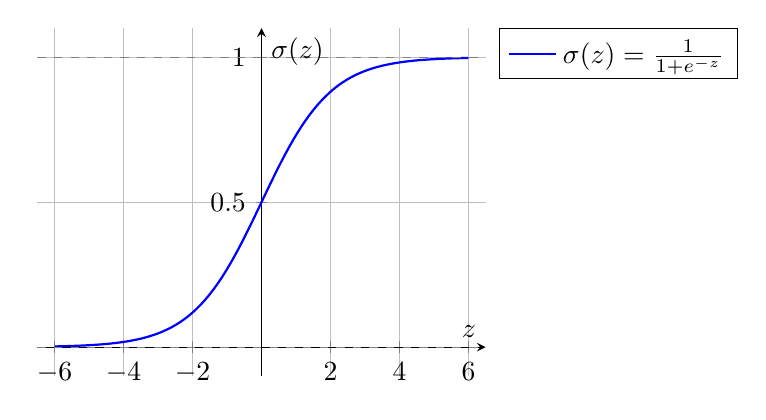
\begin{tikzpicture}
      \begin{axis}[
          width=0.6\textwidth, % Adjust width as needed
          height=6cm,
          axis lines=middle,
          xlabel={$z$},
          ylabel={$\sigma(z)$},
          grid=major,
          ymin=-0.1, ymax=1.1,
          xmin=-6.5, xmax=6.5,
          samples=100,
          domain=-6:6,
          legend pos=outer north east % Or other position
        ]
        \addplot [blue, thick] {1/(1+exp(-x))};
        \addlegendentry{$\sigma(z) = \frac{1}{1+e^{-z}}$}
        % Asymptotes
        \addplot [dashed, gray, domain=-6.5:6.5] {0};
        \addplot [dashed, gray, domain=-6.5:6.5] {1};
      \end{axis}
    \end{tikzpicture}
    \caption{The Sigmoid activation function.}
    \label{fig:sigmoid_plot}
  \end{figure}


  \paragraph{Hyperbolic Tangent Function (\( \tanh \)):}
  The hyperbolic tangent function maps any real input to the range (-1, 1). It is defined as:
  \begin{equation}
    \tanh(z) = \frac{e^z - e^{-z}}{e^z + e^{-z}} = 2\sigma(2z) - 1
  \end{equation}
  It is frequently used as the main activation function for hidden states in RNNs and LSTMs (e.g., Equations~\ref{eq:rnn_hidden_state}, \ref{eq:lstm_candidate_cell}, \ref{eq:lstm_hidden_state}). See Figure~\ref{fig:tanh_plot}.

  \begin{figure}[htbp]
    \centering
    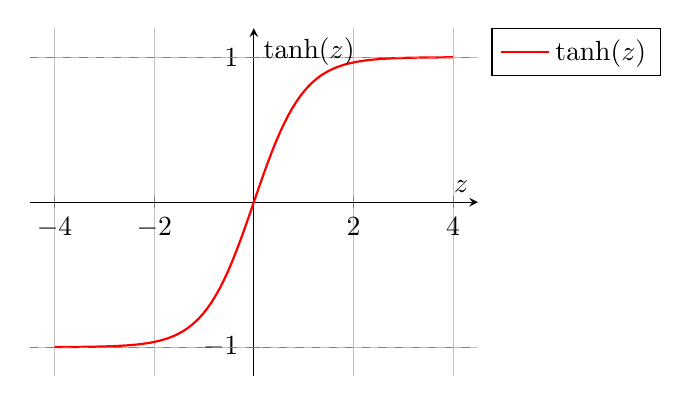
\begin{tikzpicture}
      \begin{axis}[
          width=0.6\textwidth,
          height=6cm,
          axis lines=middle,
          xlabel={$z$},
          ylabel={$\tanh(z)$},
          grid=major,
          ymin=-1.2, ymax=1.2,
          xmin=-4.5, xmax=4.5,
          samples=100,
          domain=-4:4,
          legend pos=outer north east
        ]
        \addplot [red, thick] {tanh(x)};
        \addlegendentry{$\tanh(z)$}
        % Asymptotes
        \addplot [dashed, gray, domain=-4.5:4.5] {-1};
        \addplot [dashed, gray, domain=-4.5:4.5] {1};
      \end{axis}
    \end{tikzpicture}
    \caption{The Hyperbolic Tangent (tanh) activation function.}
    \label{fig:tanh_plot}
  \end{figure}


  \paragraph{Rectified Linear Unit (ReLU):}
  The ReLU function outputs the input directly if it is positive, and zero otherwise. It is defined as:
  \begin{equation}
    \text{ReLU}(z) = \max(0, z)
  \end{equation}
  ReLU is widely used in deep learning due to its simplicity and effectiveness in mitigating the vanishing gradient problem for positive inputs. It is used within the model presented in this thesis (Section~\ref{sec:integrated_architecture} refers to the code using it). See Figure~\ref{fig:relu_plot}.

  \begin{figure}[htbp]
    \centering
    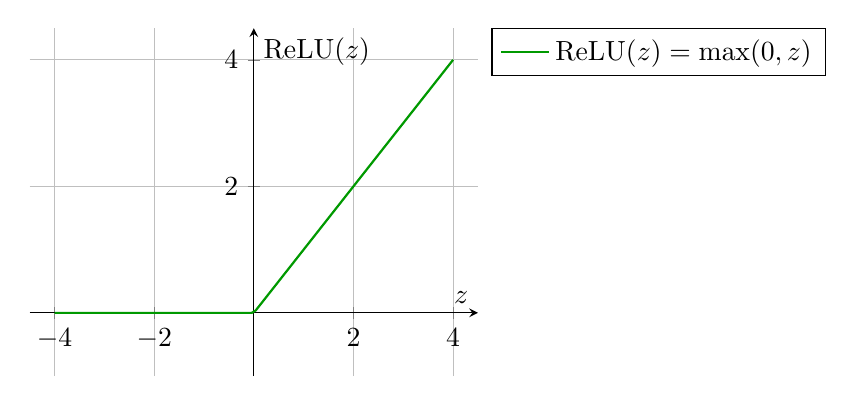
\begin{tikzpicture}
      \begin{axis}[
          width=0.6\textwidth,
          height=6cm,
          axis lines=middle,
          xlabel={$z$},
          ylabel={ReLU$(z)$},
          grid=major,
          ymin=-1, ymax=4.5,
          xmin=-4.5, xmax=4.5,
          samples=100,
          legend pos=outer north east
        ]
        \addplot [green!60!black, thick, domain=-4:4] {max(0,x)};
        \addlegendentry{ReLU$(z) = \max(0, z)$}
      \end{axis}
    \end{tikzpicture}
    \caption{The Rectified Linear Unit (ReLU) activation function.}
    \label{fig:relu_plot}
  \end{figure}


  \paragraph{Softmax Function:}
  The softmax function converts a vector of K real numbers \( \bm{z} = (z_1, ..., z_K) \) into a probability distribution consisting of K probabilities. The function is applied to the entire vector and the \( i \)-th element of the output vector is calculated as:
  \begin{equation}
    \text{softmax}(\bm{z})_i = \frac{e^{z_i}}{\sum_{j=1}^K e^{z_j}} \quad \text{for } i = 1, ..., K
  \end{equation}
  The outputs are non-negative and sum to 1 (\( \sum_{i=1}^K \text{softmax}(\bm{z})_i = 1 \)). Softmax is commonly used in the output layer of multi-class classification models and plays a crucial role in normalizing scores into attention weights in the Attention mechanism (Equation~\ref{eq:scaled_dot_product_attention}).

  % -------------------------------------------------------------------------
  \subsection{Distance and Similarity Metrics}
  \label{subsec:distance_metrics}
  % -------------------------------------------------------------------------
  These metrics quantify the difference or similarity between vectors, which is fundamental in many machine learning tasks like clustering, nearest neighbour search, and evaluating embedding spaces. Let \( \bm{a}, \bm{b} \in \mathbb{R}^d \) be two vectors of dimension \( d \).

  \paragraph{Euclidean Distance (L2 Distance):}
  \label{eq:euclidean_distance}
  The most common distance measure, representing the straight-line distance between two points in Euclidean space. It is the L2 norm of the difference between the vectors:
  \begin{equation}
    d_{\text{Euclidean}}(\bm{a}, \bm{b}) = ||\bm{a} - \bm{b}||_2 = \sqrt{\sum_{i=1}^d (a_i - b_i)^2}
  \end{equation}

  \paragraph{Manhattan Distance (L1 Distance):}
  Measures the distance by summing the absolute differences of the vector components. It corresponds to the distance travelled along axes at right angles (like navigating city blocks). It is the L1 norm of the difference:
  \begin{equation}
    d_{\text{Manhattan}}(\bm{a}, \bm{b}) = ||\bm{a} - \bm{b}||_1 = \sum_{i=1}^d |a_i - b_i|
  \end{equation}

  \paragraph{Cosine Similarity:}
  Measures the cosine of the angle between two non-zero vectors, indicating their orientation similarity irrespective of their magnitude. It ranges from -1 (exactly opposite) through 0 (orthogonal) to 1 (exactly the same direction). It is calculated using the dot product and vector magnitudes (L2 norms):
  \begin{equation}
    \text{CosineSimilarity}(\bm{a}, \bm{b}) = \frac{\bm{a} \cdot \bm{b}}{||\bm{a}||_2 ||\bm{b}||_2} = \frac{\sum_{i=1}^d a_i b_i}{\sqrt{\sum_{i=1}^d a_i^2} \sqrt{\sum_{i=1}^d b_i^2}}
  \end{equation}
  Cosine similarity is widely used for comparing high-dimensional vectors, such as text document embeddings or feature vectors, where magnitude might be less important than orientation. Note that while similarity increases as the value approaches 1, Cosine Distance is sometimes defined as \( 1 - \text{CosineSimilarity}(\bm{a}, \bm{b}) \).

  % -------------------------------------------------------------------------
  \subsection{Attention Mechanism Components}
  % -------------------------------------------------------------------------
  % (Content from previous version - Dot Product, Scaling)
  The Scaled Dot-Product Attention mechanism (Equation~\ref{eq:scaled_dot_product_attention}) relies on several fundamental operations beyond the Softmax function:

  \paragraph{Dot Product Similarity:}
  The compatibility between a query \( \bm{q} \) and a key \( \bm{k} \) (both typically vectors of the same dimension \( d_k \)) is often computed using the dot product \( \bm{q} \cdot \bm{k} = \bm{q}^T \bm{k} \). As noted above, this is closely related to Cosine Similarity but does not normalize for vector magnitudes. For matrices \( Q \) and \( K \) containing multiple queries and keys as rows, the matrix product \( QK^T \) computes all pairwise dot products efficiently.

  \paragraph{Scaling:}
  To counteract the effect of large dot product values when the dimension \( d_k \) is high, the scores \( QK^T \) are scaled down by dividing by \( \sqrt{d_k} \) before applying the softmax function. This helps maintain a stable gradient flow during training.

  % -------------------------------------------------------------------------
  \subsection{Normalization Techniques}
  % -------------------------------------------------------------------------
  Normalization layers help stabilize training, speed up convergence, and sometimes improve generalization by standardizing layer inputs.

  \paragraph{Layer Normalization (LayerNorm):}
  Layer Normalization normalizes the inputs across the features for \textit{each individual data sample} in a batch, making its computation independent of the batch size. For an input vector \( \bm{x} \) representing the features for one sample at a specific layer, LayerNorm computes:
  \begin{equation}
    \text{LayerNorm}(\bm{x}) = \bm{\gamma} \odot \frac{\bm{x} - \mu_{\text{sample}}}{\sqrt{\sigma^2_{\text{sample}} + \epsilon}} + \bm{\beta}
    \label{eq:layernorm}
  \end{equation}
  Here, \( \mu_{\text{sample}} \) and \( \sigma^2_{\text{sample}} \) are the mean and variance calculated across the feature dimension(s) of the single input sample \( \bm{x} \). \( \bm{\gamma} \) (scale) and \( \bm{\beta} \) (shift) are learnable affine transformation parameters of the same dimension as \( \bm{x} \), and \( \epsilon \) is a small constant added for numerical stability. LayerNorm is frequently used in RNNs and Transformers (including the model implemented in this work) where batch statistics might be less stable or meaningful.

  \paragraph{Batch Normalization (BatchNorm):}
  (Included for contrast, delete if not relevant) Batch Normalization normalizes inputs across the \textit{batch dimension} for each feature separately. It calculates the mean \( \mu_{\text{batch}} \) and variance \( \sigma^2_{\text{batch}} \) for each feature across all samples in the current mini-batch. While highly effective in CNNs, its dependence on batch statistics can be less suitable for sequence models with variable lengths or small batch sizes compared to LayerNorm.

  % -------------------------------------------------------------------------
  \subsection{Pooling Strategies for Sequences}
  % -------------------------------------------------------------------------
  Pooling layers are used to aggregate information across the time or sequence dimension, often to produce a fixed-size representation from variable-length sequence outputs for downstream tasks like classification. Given a sequence of hidden states \( H = [\bm{h}_1, \bm{h}_2, ..., \bm{h}_T] \), where each \( \bm{h}_t \in \mathbb{R}^d \):

  \paragraph{Mean Pooling:}
  Calculates the element-wise average of the hidden state vectors across the sequence dimension:
  \begin{equation}
    \bm{h}_{\text{mean\_pool}} = \frac{1}{T} \sum_{t=1}^T \bm{h}_t
  \end{equation}
  The resulting vector \( \bm{h}_{\text{mean\_pool}} \in \mathbb{R}^d \) represents the average activation over the sequence. This strategy is used in the implemented model to summarize the output sequence before the final classification layer.

  \paragraph{Max Pooling:}
  Calculates the element-wise maximum of the hidden state vectors across the sequence dimension:
  \begin{equation}
    (\bm{h}_{\text{max\_pool}})_j = \max_{t=1...T} (\bm{h}_t)_j \quad \text{for } j = 1, ..., d
  \end{equation}
  The resulting vector \( \bm{h}_{\text{max\_pool}} \in \mathbb{R}^d \) captures the strongest activation for each feature dimension across the sequence.

  % -------------------------------------------------------------------------
  \subsection{Weight Initialization}
  % -------------------------------------------------------------------------
  Initializing the weight parameters of a neural network appropriately is crucial for effective training, helping to prevent issues like vanishing or exploding gradients.

  \paragraph{Kaiming (He) Initialization:}
  Proposed by He et al. \autocite{he2015delving}, this method is primarily designed for layers followed by Rectified Linear Unit (ReLU) activations. It accounts for the non-linearity of ReLU. For Kaiming Normal initialization (used in the implemented model via `kaiming_normal_`), weights \( W \) are drawn from a normal distribution \( \mathcal{N}(0, \text{std}^2) \), where:
  \begin{equation}
    \text{std} = \sqrt{\frac{2}{\text{fan\_in}}}
  \end{equation}
  Here, `fan_in` is the number of input units to the weight tensor. A variant considers the non-linearity slope \( a \) of leaky ReLU (where \( a=0 \) for standard ReLU).

  \paragraph{Xavier (Glorot) Initialization:}
  Proposed by Glorot and Bengio \autocite{glorot2010understanding}, this method aims to keep the variance of activations and gradients roughly constant across layers, particularly effective for symmetric activations like tanh or sigmoid. For Xavier Normal initialization, weights \( W \) are drawn from \( \mathcal{N}(0, \text{std}^2) \), where:
  \begin{equation}
    \text{std} = \sqrt{\frac{2}{\text{fan\_in} + \text{fan\_out}}}
  \end{equation}
  `fan_out` is the number of output units. Uniform versions also exist for both Kaiming and Xavier initialization.

  % -------------------------------------------------------------------------
  \subsection{Optimization Algorithms and Refinements}
  % -------------------------------------------------------------------------
  Optimization algorithms iteratively update model parameters \( \theta \) to minimize a loss function \( J(\theta) \).

  \paragraph{Stochastic Gradient Descent (SGD):}
  A fundamental algorithm that updates parameters based on the gradient of the loss computed on a small batch (or single sample) of data at iteration \( k \).
  \begin{equation}
    \theta_{k+1} = \theta_k - \eta \nabla J(\theta_k; \bm{x}^{(i)}; \bm{y}^{(i)})
  \end{equation}
  where \( \eta \) is the learning rate and \( \nabla J(...) \) is the gradient computed on a mini-batch \( (\bm{x}^{(i)}, \bm{y}^{(i)}) \). Variants include momentum or Nesterov momentum.

  \paragraph{Adam Optimizer:}
  \label{eq:adam}
  An adaptive learning rate optimization algorithm that computes individual adaptive learning rates for different parameters using estimates of first and second moments of the gradients \autocite{kingma2014adam}. It often converges faster than basic SGD. The update rules involve computing biased moment estimates (\( \bm{m}_t, \bm{v}_t \)), bias-corrected estimates (\( \hat{\bm{m}}_t, \hat{\bm{v}}_t \)), and then updating parameters:
  \begin{equation}
    \theta_{t+1} = \theta_t - \frac{\eta}{\sqrt{\hat{\bm{v}}_t} + \epsilon} \hat{\bm{m}}_t
    \label{eq:adam-update} % Reuse label if needed
  \end{equation}
  Adam is used for training the model in this work.

  \paragraph{Learning Rate Scheduling:}
  Techniques used to adjust the learning rate \( \eta \) during training, which can improve convergence and final model performance.
  \begin{itemize}
    \item \textit{ReduceLROnPlateau:} Monitors a specified metric (e.g., validation loss). If the metric does not improve for a defined number of 'patience' epochs, the learning rate is reduced by a multiplicative 'factor'. This strategy is employed in the training procedure of this thesis.
    \item \textit{Step Decay:} Reduces the learning rate by a fixed factor every specified number of epochs.
    \item \textit{Cosine Annealing:} Gradually decreases the learning rate following a cosine curve shape over a specified number of epochs or iterations.
  \end{itemize}

  % -------------------------------------------------------------------------
  \subsection{Loss Functions}
  % -------------------------------------------------------------------------
  % (Content from previous version - MSE, BCE, CCE - keep only relevant ones)
  Loss functions quantify the difference between the model's predictions and the true target values, guiding the optimization process.

  \paragraph{Binary Cross-Entropy (BCE):}
  \label{eq:bce} % Reuse label if needed
  Used for binary classification tasks where the model outputs a probability \( \hat{p}_i \) for the positive class (true label \( y_i \in \{0, 1\} \)). It is the loss function used in the model training for this thesis.
  \begin{equation}
    \text{BCE} = -\frac{1}{N} \sum_{i=1}^N [ y_i \log(\hat{p}_i) + (1 - y_i) \log(1 - \hat{p}_i) ]
  \end{equation}

  % Remove MSE/CCE if not used elsewhere in the thesis

  % -------------------------------------------------------------------------
  \subsection{Regularization Techniques}
  % -------------------------------------------------------------------------
  % (Content from previous version - L2, Dropout)
  Regularization techniques are used to prevent overfitting by adding constraints or penalties to the model or its training process.

  \paragraph{L2 Regularization (Weight Decay):}
  Adds a penalty to the loss function proportional to the squared magnitude of the model weights \( \theta \).
  \begin{equation}
    J_{reg}(\theta) = J(\theta) + \frac{\lambda}{2} ||\theta||_2^2 = J(\theta) + \frac{\lambda}{2} \sum_i \theta_i^2
  \end{equation}
  where \( \lambda \) is the regularization strength. This encourages smaller weights.

  \paragraph{Dropout:}
  During training, randomly sets a fraction of neuron activations (outputs) to zero at each forward pass before the subsequent layer \autocite{srivastava2014dropout}. This prevents units from overly co-adapting and can be interpreted as training an ensemble of thinned networks. The dropout rate (e.g., 0.3 in the implemented model) specifies the probability of an element being zeroed out. At test time, dropout is turned off, and sometimes the outputs of the kept units are scaled down by the dropout rate (though often handled implicitly by libraries or absorbed into subsequent layers). Dropout is used in both the LSTM layers and the final fully connected block in the implemented model.

  % -------------------------------------------------------------------------
  \subsection{Data Handling for Sequences}
  % -------------------------------------------------------------------------

  \paragraph{Sequence Padding:}
  Neural networks typically require inputs within a batch to be tensors of uniform shape. Since sequential data (like manufacturing process steps or natural language sentences) often has varying lengths, techniques are needed to handle this during batch processing. Padding involves augmenting shorter sequences within a batch with special padding values (often zero) until they reach the length of the longest sequence in that batch. This results in rectangular tensors suitable for processing. The `collate_fn` used in the data loading pipeline for this thesis employs padding (via `pad_sequence`). It is important that subsequent computations (e.g., loss calculation, attention mechanisms) are designed to ignore or mask these padded values to avoid introducing noise.

\end{appendices}